\section{Composition of dynamic verbs via temporal anaphora}
\marginnote{\textcolor{blue}{Postscript: with the exception of entification and metaphor, all of these sketches are things I had in mind while initially writing the thesis but didn't make it to the submitted version, so there will probably be technical errors, but this shouldn't compromise the sketches because they are not intended to be rigorous. None of these sketches (and nothing else in this thesis for that matter) should be taken as canonical once-and-for-all solutions to the conceptual problems they are meant to tackle; they are more meant to provoke as first-pass attempts, and they are meant to demonstrate how to play around and have fun in \textbf{ContRel} with string diagrams. I'll also note here that everything in \textbf{ContRel} is a kind of truth-conditional possible worlds semantics (up to some arbitrary but fixed choice of what particular ensembles of shapes and movements the modeller supplies up front), so there are no guarantees about how any of this material would fare if one tried to take the diagrams and interpret them in terms of neural networks, and I make no claims about whether the mathematics reflects actual cognition. However, I will claim that these mathematical sketches reflect at least the phenomenology of how \emph{I} think about language, which should come as no surprise because my methodology was armchair introspection.}}
Dynamic verbs in iconic semantics may be modelled by homotopies, but non-parallel composition of homotopies is only defined up to parameters with indications of how the two separate homotopies begin and end relative to one another; i.e. temporal data.

\begin{example}[Gluing homotopies sequentially at a time $\gamma \in (0,1)$]

\end{example}

The technical difficulty I'd like to sketch a solution for is that while these parameters must be given as real numbers in the interval $[0,1]$, temporal natural language underspecifies: e.g. in the utterance \texttt{Bob drank, and then he slept} he could have drank in the morning and then slept in the afternoon, or both in the evening, and so on. The easy solution is to have absolute temporal anchors, but we seem to get by with less, which appears to necessitate a possible-worlds approach. Arguably the theoretical minimum we require is a kind of algebra for temporal aspects as in Yucatan [CITE], so here I sketch an algebra for temporal anaphora in \textbf{ContRel} that only requires copy-delete along with the standard topology on $\mathbb{R}$ obtained by the encoding of intervals as the open set $<: [0,1] \times [0,1]$. Then I'll show how this temporal data can be used to supply the information required for homotopy composition, which should indicate that \textbf{ContRel} is in-principle sufficiently expressive for dynamic iconic semantics for natural language, i.e. the interpretation of text as little moving cartoons.

\begin{defn}[A sketch text-circuit algebra for temporal anaphora]
We consider three kinds of events. The first is episodic, which corresponds to some interval on $[0,1]$ with endpoints $t_{\texttt{EV}}^0$ and $t_{\texttt{EV}}^1$. We model these as bipartite states with the initial constraint that $t_{\texttt{EV}}^0 < t_{\texttt{EV}}^1$. The second is habitual, which could in principle be an arbitrary subset of $[0,1]$, but there are pathologies we would like to rule out as a matter of common sense (e.g. we don't really talk about events that occur in time according cantor set), so we treat habituals as open sets (unions of intervals) to be later constructed or supplied as constraints; when we are finished specifying the algebra, equipping it with unions as a kind of formal sum will approximate those open sets that are constructible by finite amounts of talking about times. The third is a hybrid of the first two, where we consider some open set with distinguished endpoints, modelled as a restriction/intersection of an interval with some other open set.
\[\tikzfig{time/episodic}\]
Now we model temporal aspects as circuit components --- what appears to distinguish aspects from tenses is that aspects are always relative to the temporal data of two events, whereas tenses may be "intransitive" on events --- so all of our aspectual data will involve constraining pairs of events (one of which is a \texttt{TOPIC}). The first kind of aspect we consider is \emph{perfective}, which constraints an event time to be within topic time; we model this as imposing a constraint that the endpoints of the event must lie within the interval specified by the endpoints of the topic. In discourse, introducing a perfective constraint corresponds to adding a gate.
\[\tikzfig{time/perf}\]
The \emph{terminative} aspect constrains an event to occur entirely before the beginning of the topic time. Terminative composition of verbs may be glossed as \texttt{(event) and-then (topic)}, and this kind of composition yields the view of text circuits as implicitly encoding the temporal order in which gate-as-events occur, where now the sequential ordering of gates matters. This failure of interchange interprets text circuits in something like a premonoidal setting [CITE].
\[\tikzfig{time/terminative}\]
The \emph{imperfective} aspect we consider as constraining an episodic topic time to lie within some ongoing habitual event, where the habitual event is represented as a free coparameter. In discourse, introducing an imperfective constraint corresponds to splicing in such a constraint, which we gloss as a gate that restricts the endpoints of the topic interval to lie within the open set representing the habitual event time as a coparameter. We skip over the subtly distinct \emph{progressive} aspect here as we won't need it for our later example, but it should be clear that an approach along these lines will also suffice.
\[\tikzfig{time/imperf}\]
\end{defn}

\begin{example}
So here is an example of Yucatan Maya taken from [CITE], which is an excerpt of an interview with a speaker fleeing a cyclone. I have split the excerpt into numbered single-verb clauses, accompanied by glosses in English with aspect-markers and the corresponding evolution of a text-circuit by the discourse rewrites we have defined. The first event introduced into discourse is the arrival of the refugees in the village, which is marked as perfective.
\[(1) \quad \left[ \begin{array}{c}\texttt{\emph{Kaajk'ucho'on} t\'{u}un way tek\`{a}ajil x Jaxleyile,} \\ \hline \texttt{When we }\underbrace{\texttt{\emph{arrived}}}_{\textsc{\makebox[0pt]{PERF.}}}\texttt{,}\end{array} \right] \vcenter{\scalebox{0.75}{\tikzfig{time/ex0}}}\]
The second event is what the refugees saw, implicitly concurrent with event (1), which we opt to treat with a prepended copy of endpoints. \texttt{arrive \& see} then form an atomic topic for events (3) and (4), which we deal with by constraining both (1) and (2) in the same way. Note that there is a single variable open set $t_\texttt{say}$ that is repeated 4 times in the diagram.
\[(2) \quad \left[ \begin{array}{c} \texttt{\emph{kilike'} tul\'{a}akal m\'{a}ake',} \\ \hline \texttt{we } \underbrace{\texttt{\emph{saw}}}_{\textsc{\makebox[0pt]{PERF.}}}\texttt{,} \end{array} \right] \quad \vcenter{\scalebox{0.75}{\tikzfig{time/ex1}}}\]
The third event refers to the villagers saying something, in the imperfective aspect with respect to events (1) and (2), so we constrain those topics accordingly. In gloss, it was an ongoing event that the villagers were saying something when the refugees arrived.
\[(3) \quad \left[ \begin{array}{c} \texttt{\emph{t\'{a}an uya'aliko'obe'} jach} \\ \hline \texttt{everyone }\underbrace{\texttt{\emph{was saying}}}_{\textsc{\makebox[0pt]{IMPF. wrt. (1,2)}}}\end{array} \right] \quad \vcenter{\scalebox{0.75}{\tikzfig{time/ex2}}}\]
The fourth event refers to what the villagers had heard, in the terminative aspect with respect to (1) and (2). In gloss, the villagers were saying (reporting) the episodic event of them hearing something on the radio, and this hearing-event had completed before the refugees' arrival.
\[(4) \quad \left[ \begin{array}{c} \texttt{\emph{ts'uyu'ubiko'ob ti'} r\`{a}adyoe'} \\ \hline \texttt{(they) }\underbrace{\texttt{\emph{had heard }}}_{\textsc{\makebox[0pt]{TERM. wrt. (1,2)}}}\texttt{on the radio} \end{array} \right] \quad \vcenter{\scalebox{0.75}{\tikzfig{time/ex3}}}\]
The fifth event refers the coming of the cyclone, which was ongoing at the time of the villagers hearing the radio report. This introduces a new habitual event as the variable open set $t_\texttt{come}$, repeated twice in the diagram as constraints.
\[(5) \quad \left[ \begin{array}{c} \texttt{\emph{t\'{u}un t\`{a}al} le sikl\`{o}ono'.} \\ \hline \texttt{the cyclone }\underbrace{\texttt{\emph{was coming.}}}_{\textsc{\makebox[0pt]{(4) IMPF. wrt. (5)}}} \end{array} \right] \quad \vcenter{\scalebox{0.75}{\tikzfig{time/ex4}}}\]
Altogether, the final diagram represents a map from two open sets on $[0,1]$ (representing the potentially habitual events \texttt{say} and \texttt{come} encoded as variable open sets $t_\texttt{say}$ and $t_\texttt{come}$) to return a state in \textbf{ContRel} that encodes the set of possible endpoints for the episodic events \texttt{arrive}, \texttt{see} and \texttt{hear}: $\{(t_\texttt{arrive}^0,t_\texttt{arrive}^1,t_\texttt{see}^0,t_\texttt{see}^1,t_\texttt{hear}^0,t_\texttt{hear}^1)\}$. Moreover, we have set up the algebra to allow us to leverage compositional discourse structure in such a way that sampling any of the elements of the resultant set returns a choice of endpoints consistent with the temporal constraints of the excerpt.
\end{example}

\newpage
\section{Iconic semantics for modal verbs}

In this sketch I want to deal with certain modal verbs: that means those of cognition and perception like to think and see, and the sketch will taper out towards some modal auxiliaries like wanting. These kinds of verbs are roughly characterised as requiring copies of entities to be instantiated in worlds similar to but not exactly that of whatever base narrative reality is referred to in the discourse. For example, in \texttt{Alice sees Bob drink a beer, Bob drinks another after Alice leaves.}, there are two Bobs, because the one in Alice's mental-theatre drinks a single beer, and the one in the base reality of the narration drinks two. So there are two worlds $\mathfrak{W}$ here, one basic, and a $\mathfrak{W}_{\texttt{A}}$ for the world in Alice's perception. Things get intractably tricky fairly quickly with these modals: to do epistemic logic means to have nested indices of what Alice thinks Bob thinks Alice thinks, to gossip is to reason about he-said-she-said, to understand complex narratives is to reason about stories-told-within-stories, and counterfactuals are a whole thing too. So that is a fundamental mystery: all this seems fairly complicated to encode and reason about symbolically, but it is phenomenologically fairly easy for adults to do, so what gives? What sort of mathematical presentation of these modals would at least reflect this lightness and ease?

I think thought-bubbles that show up in comic books are a pretty good start. Their cloudlike shape is a visual convention indicating a separate mental world, and they are typically used to represent want when the contents are also iconic representations.

\begin{figure}[h!]
    \centering
    \begin{minipage}[b]{0.4\textwidth}
        \centering
        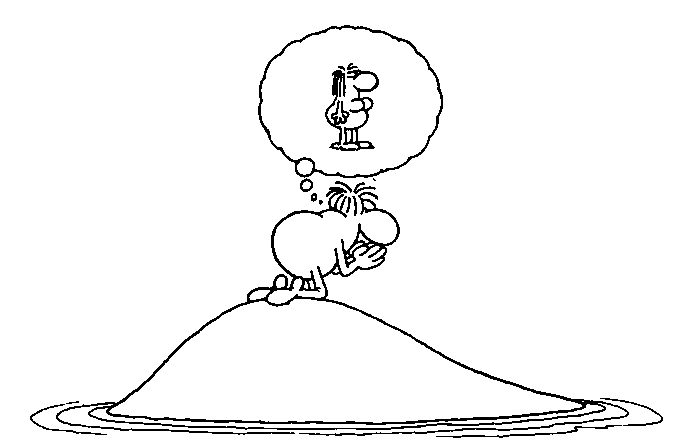
\includegraphics[height=4cm]{figures/bubbles/companion}
        \label{fig:companion}
    \end{minipage}
    \hfill
    \begin{minipage}[b]{0.4\textwidth}
        \centering
        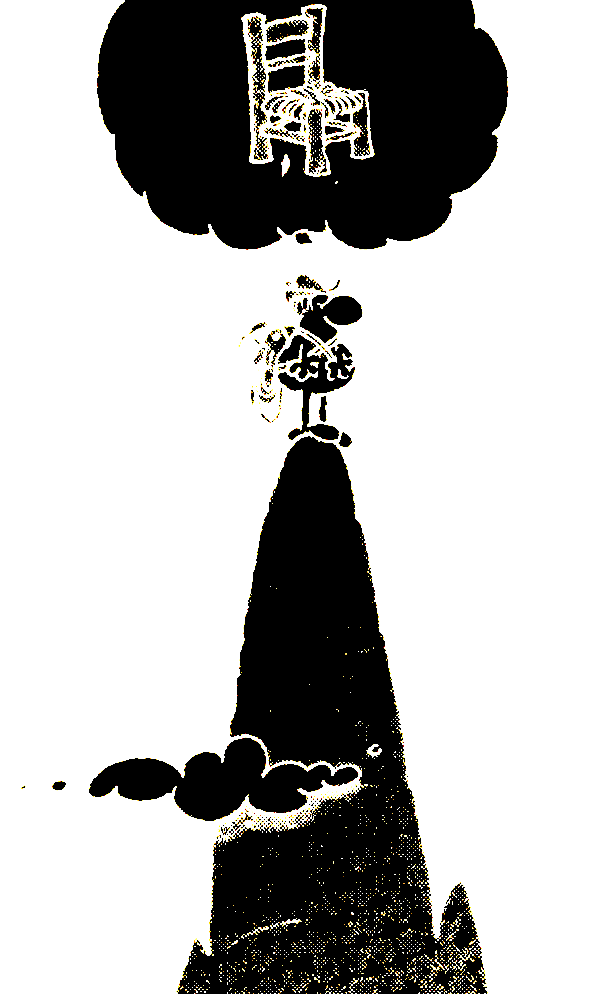
\includegraphics[height=4cm]{figures/bubbles/chair}
        \label{fig:chair}
    \end{minipage}
    \caption{Two examples by Mordillo, an artist I liked as a child: a thought bubble representing a woman, where the context of a stranded man implies a want for companionship, and a thought bubble representing a chair, where the context of a climber on a tall summit implies a want for rest.}
    \label{fig:mordillo}
\end{figure}

The visual convention for cognitive and perceptive-alethic verbs is, as far as I can tell, a kind of x-ray effect into the contents of a head, which employs the familiar container metaphor: the head is a container for thoughts.

\begin{figure}[h!]
    \centering
    \begin{minipage}[b]{0.4\textwidth}
        \centering
        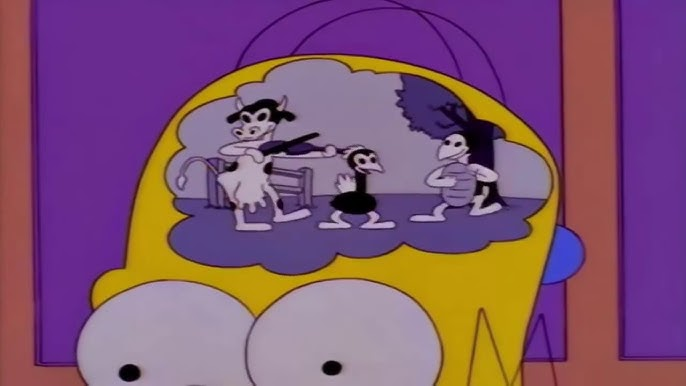
\includegraphics[height=4cm]{figures/bubbles/homer}
        \label{fig:homer}
    \end{minipage}
    \hfill
    \begin{minipage}[b]{0.4\textwidth}
        \centering
        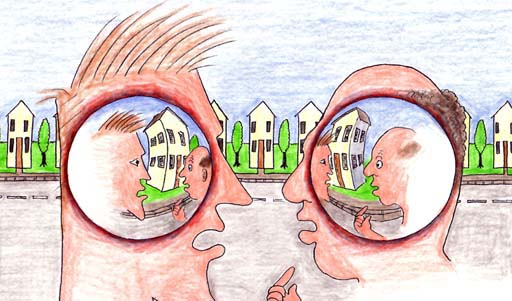
\includegraphics[height=4cm]{figures/bubbles/nestedminds}
        \label{fig:lehar}
    \end{minipage}
    \caption{On the left, a scene from the Simpsons showing the contents of Homer's mental-theatre. On the right, a depiction of two separate mental-theatres with a fisheye effect, taken from Steven Lahars "A Cartoon Epistemology" freely available online, which was also the initial inspiration for this sketch.}
    \label{fig:thinking}
\end{figure}

\begin{figure}[h!]
    \centering
    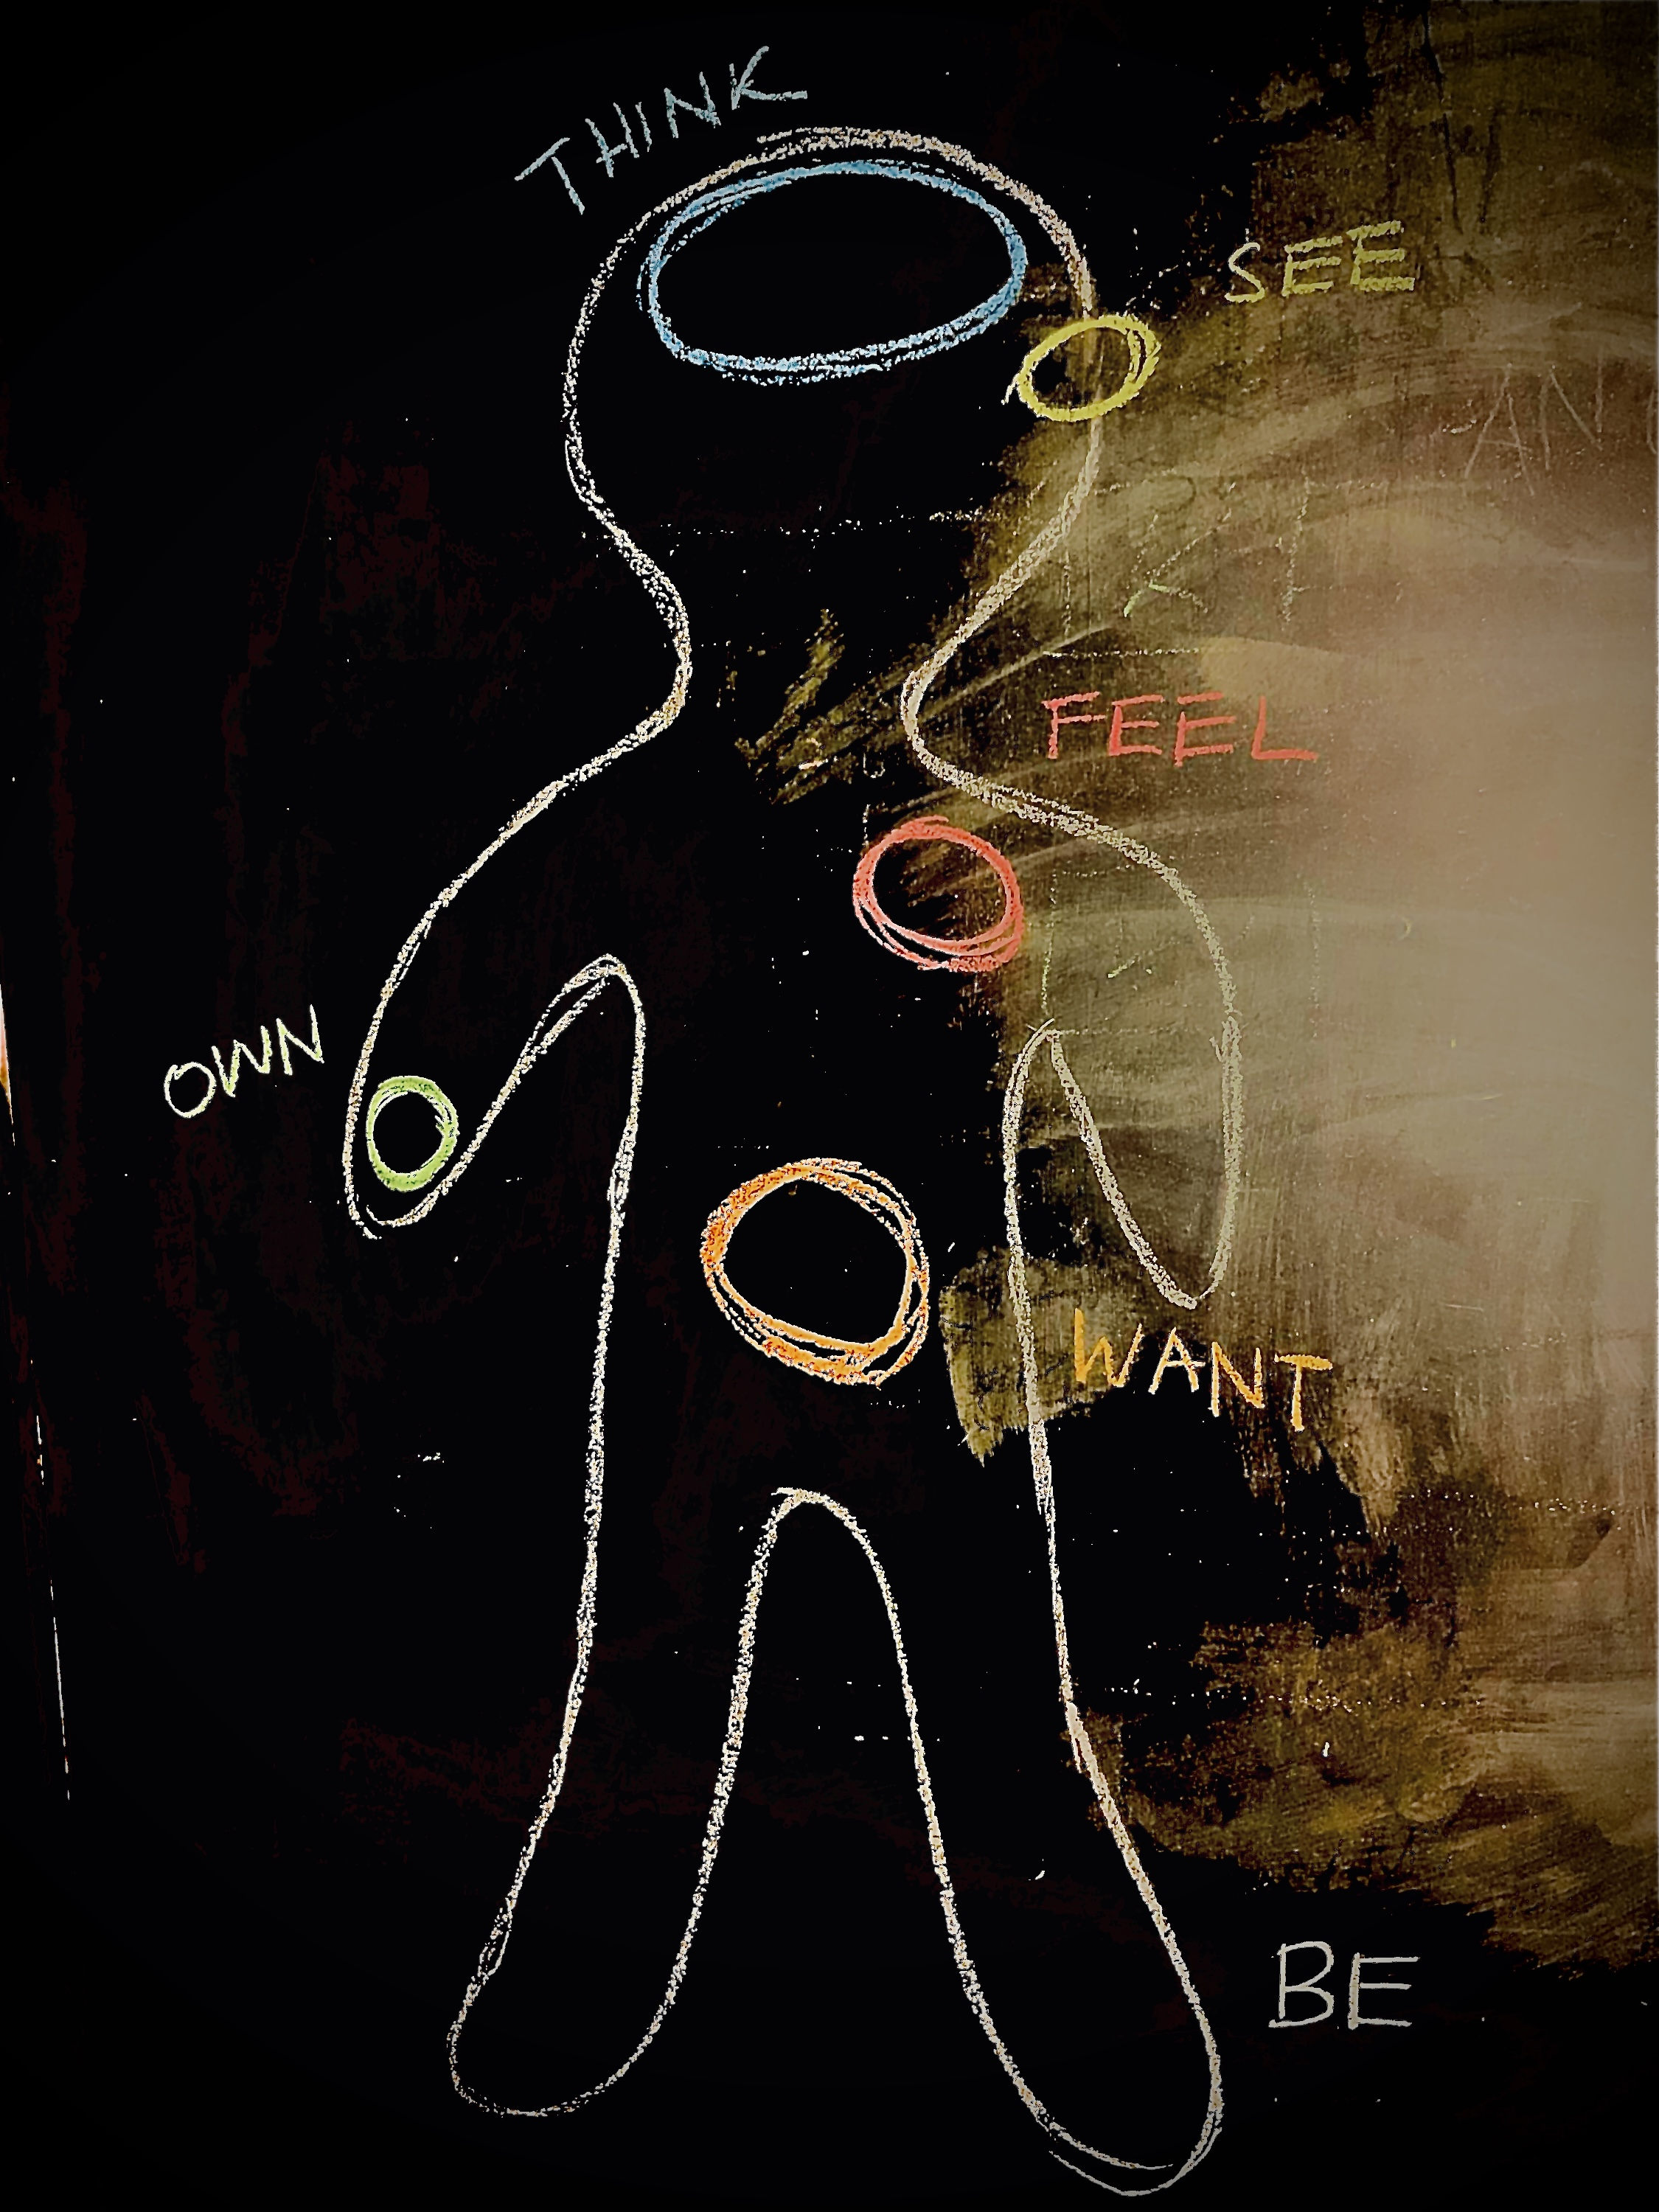
\includegraphics[height=9cm]{figures/bubbles/creepy}
    \caption{So the basic idea is to put representations of worlds inside bounded regions as containers, and in this way iconic semantics provides a univocal setting that displays all of the relevant worlds at once. We are free to pick visual conventions, as they are no more or less arbitrary than the assignment of indices and symbols such as $\mathfrak{W}_{\texttt{A}}$ to the contents of possible worlds. Here is a sketch convention for containers on an iconic representation of a person for different modal verbs: seeing, thinking, feeling, owning, and wanting. I sent this excitedly with little supporting context to Bob while I was writing my thesis. He was concerned. Then I got concerned. Childlike became creepy, and neither are good looks. I think I have supplied enough context to make this sensible, but there's no way I'm going to beat the crazy allegations.}
    \label{fig:creepy}
\end{figure}

For alethic verbs in particular (those modals that are truth-preserving, in that they "do not forget" the truth), there's a need for the contents of the container to be synchronised with the contents of the outside world. Here are some observations that enable this in \textbf{Contrel}. The basic enabling insight is that, in Euclidean spaces, if we have a hollow container with a solid blob inside, there's an approximately continuous bijection between the (open set) insides of the container and the outside world.

\clearpage

\begin{figure}[h!]
\centering
\[\scalebox{0.75}{\tikzfig{bubbles/container}}\]
\caption{The inside and the outside of a container with a solid blob inside are both homotopic to the space with a puncture. This is only approximately a continuous bijection because the unbounded outside space can only map to the open interior of the container. We can use such bijections as a bridge to establish connections between elements of different possible worlds.}
\label{fig:creepy}
\end{figure}

The second, and unfinished, idea is that if we have a handle on the individual components of sticky spiders, then we may use something like a very-well-behaved lens (hence its occurrence in the introduction) to ensure that the inside of the container is really behaving like a faithful storage medium for the goings-on outside. I think that's suggestive enough, and I'll deal with parthood in the next sketch. The last thing I want to deal with here is the problem of infinite regress for epistemic modals like knowing: if I know something, then I know I know it, and I know I know I know it, and so on. A na\"{i}ve solution is to just use an infinitely-nested series of containers.

\begin{figure}[h!]
\centering
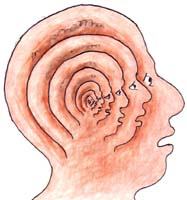
\includegraphics[height=5cm]{figures/bubbles/infinity}
\caption{Again from Cartoon Epistemology, on the unsatisfactory nature of infinitely-nested containers: \emph{But who is the viewer of this internal theatre of the mind? For whose benefit is this internal performance produced? Is it the little man at the center who sees this scene? But then how does HE see? Is there yet another smaller man inside that little man's head, and so on to an infinite regress of observers within observers?}}
\label{fig:infinity}
\end{figure}

\clearpage

So the problem here is how to encode this infinite regress with finite means in an iconic model. The usual monadic approach still runs into the problem that you have to map a potential nested-infinity of possible worlds onto some finite model if one cares about cognitive realism. In iconic semantics, we can modify the space itself; here I think Escher was onto something.

\begin{figure}[h!]
\centering
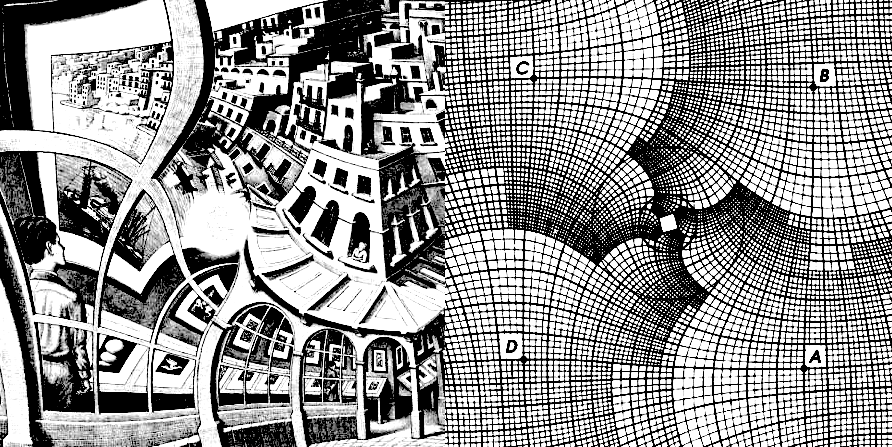
\includegraphics[height=8cm]{figures/bubbles/combined}
\caption{Escher's "Print Gallery" lithograph alongside his working sketch of the vortex-grid geometry the work was built on. On the left of the lithograph, an observer examines a framed painting of a town. Going clockwise, we see more details of the town, which has in it a print gallery, within which is the original observer. The missing centre of the piece where Escher signed the work obscures what would have been infinite nesting; the right-hand-side of the frame would have spiraled along the vortex infinitely. Treating the frame as a container, here we have an example of a container that contains itself, where movement clockwise indicates going down a level, clockwise going up, yet no explicit infinities anywhere.}
\label{fig:gallery}
\end{figure}

The space in which such an arrangement can be realised is the same as that of the Penrose staircase: splitting the lithograph into four corners, each is a locally consistent snapshot, each gluing of quadrants is a consistent (as/de)scent, but the overall manifold obtained needs to be embedded in a higher dimension. While this in principle solves the problem of finitely representing infinite descent, these kinds of spaces are not grounded in physical, embodied intuitions. I think it is mathematically neat that there can exist topological models for such modal verbs, but whether such proposals are to be taken seriously as modelling cognition is a thorny matter I don't want to say more about.

\newpage
\section{Breaking shapes into parts and gluing them back together}

Containers ought to be able to open up so things can be put in them, but at the moment our shapes are static and solid, so we can't simply phase objects into containers by sliding them around in flatland. So in this sketch, I want to explore parthood; how to move around the individual shapes of a sticky-spider, how to shatter one of these component shapes into parts that can move independently of one another, and how to glue them back together again. Let's assume for simplicity that we only want to deal with \emph{nice} sticky-spiders where cores and halos agree and are both contractible opens; i.e. the spider can be expressed as a finite union of open solid blobs as effects followed by the same open solid blob as a state.

\begin{defn}[Nice sticky-spiders]
A sticky-spider is \emph{nice} if it is equal to a union of contractible open effects followed by the same contractible open expressed as a state.
\[\tikzfig{topology/nicespider}\]
\end{defn}

Let's also say we start with the ability to detect whether two sticky-spiders are related to one another by rigid displacements, expressed as a topological group with elements we denote $\rho$. Since sticky-spiders can be represented as unions of effects followed by states, we can define a binary relation on sticky-spiders that tells us whether they are the same up to rigidly displacing component shapes:

\begin{defn}[Displacement relation]
Two sticky-spiders (cyan and green, both assumed to be nice here), each with components indexed by $I$, are \emph{equivalent up to displacement} when there exist $\rho_i$ such that:
\[\tikzfig{topology/displacementrelation}\]
We've suppressed labelling of the states and we've contracted the cup to just depict the open state as a semicircle.
\end{defn}

Displacement is evidently an equivalence relation, and moreover requires that the two spiders related have the same number of components. Now given a particular nice spider, we treat its equivalence class of spiders as a configuration space in which we have access to all of its rigidly displaced variants at once.

\begin{defn}\label{defn:configurationspace}
The \emph{configuration space} $C(\mathfrak{s})$ of a nice spider $\mathfrak{s}$ with indexing set $I$ is the topological space with underlying set defined to be the equivalence class $[\mathfrak{s}]$ of $\mathfrak{s}$ under displacement. Assuming the topological group of rigid displacements is itself a topological space $G$, the topology of $C(\mathfrak{s})$ is a restriction of $\bigtimes^{|I|} G$ to those $|I|$-tuples of displacements witnessed by $[\mathfrak{s}]$.
\end{defn}

In configuration spaces we're making use of the fact that any displacement relationship comes with a witnessing tuple of $\rho_i$s. As a consequence, the configuration space of a sticky-spider is a retract of the product space $\bigtimes^{|I|} G$ where $G$ is the topological group of displacements.

We can depict the \emph{configuration space} of shapes that are obtainable by displacing the shapes of a given spider by a split idempotent through the n-fold tensor of rigid transformations -- a restriction to the subspace of the largest open set contained in the subset of all valid (with correct chirality) combinations of displacements that yield another spider; points in configuration space are sticky spiders related to each other by rigid transforms. Note that as a subspace, the retract of the idempotent is a function. The section and retract pair is not unique; they may for instance encode a choice of basepoint for each shape relative to which the displacement of that shape occurs.
\[\tikzfig{topology/configurations}\]
The data of rigid motion on a sticky spider as we have defined above can be captured as a continuous map from the unit interval to the space of rigid transformations; continuous paths in configuration space model motions of shapes in space.
\[\tikzfig{topology/rigidmotion2}\]
\end{defn}

\begin{defn}[Slideability in flatland]\label{defn:sliding}
What we mean by two sticky spiders being relatable by sliding shapes is that we have a homotopy that begins at one and ends at the other, such that every point in between is itself a sticky spider related to the first by rigid displacement.
\end{defn}

\begin{figure}[h!]
\centering
\[\resizebox{\textwidth}{!}{\tikzfig{topology/rigidmotion}}\]
\caption{Depicting homotopies as hexagons, two sticky-spiders (starting with cyan and ending with green) are slidably related if they are the endpoints of a homotopy (the top two conditions), and if at every point in time in the homotopy, there exists a rigid displacement $\rho_i$ for each component shape $i$ of the initial spider such that the result of the homotopy at that point in time is also a sticky-spider (expressed in union-form) that is obtainable by rigidly displacing the component shapes of the initial sticky-spider with respect to $\rho_i$. We'll further ask that the $\rho_i$ are obtained by a continuous function from $[0,1]$, to prevent discrete jumps.}
\end{figure}

Now suppose we start with a sticky-spider and we consider the space of all sticky-spiders that are slideably related; this gives us a configuration space of the original spider, where each point in the space corresponds to a spatial reconfiguration up to rigid displacement of the component shapes of the original spider.



\begin{myboxR}
\begin{example}[The connected components of configuration space]
What are the connected components of configuration space? Evidently, there are pairs of spiders that are both valid displacements, but not mutually reachable by rigid motion. For example, shapes might \emph{enclose} or \emph{trap} other shapes, or shapes might be \emph{interlocked}. Depicted are some pairs of configurations that are mutually unreachable by rigid transformations. Now we have the conceptual toolkit to begin modelling these concepts in the configuration space of a sticky spider.
\[\tikzfig{topology/encloseexample}\]
\end{example}
\end{myboxR}


\begin{myboxB}
\begin{defn}[Parthood]\label{defn:parthood}
Let's say that a "part" refers to an entire simply connected component. Simply connected is already a concept in our toolkit. A shape $U$ is disjoint from another shape $V$ intuitively when we can cover $U$ in a blob with no holes such that the blob has no overlap with $V$. So, $U$ is a part of $V$ when it is simply connect, wholly contained in $V$, and there exists a contractible open that is disjoint from $V$ that covers $U$. Diagrammatically, this is:
\[\tikzfig{topology/parthood}\]
\end{defn}

\end{myboxB}